\chapter{Results: Imaging}
\label{imaging}

Results presented in Chapter 4 determined the ideal conditions for imaging small numbers of Ba atoms in SXe.  Ideal excitation wavelengths were determined by studying the excitation spectra of the signal as well as the background.  Bleaching of the fluorescence determined ideal laser intensities to be used.  Studies of deposits made and observed at different temperatures informed the procedure of depositing at $50 \pm 5$~K and observing at 11~K.  Imaging of the 577- and 591-nm fluorescence is presented in \ref{sec:imaging590and577} down to the $10^{4}$-atom level, and imaging of the 619-nm peak is presented down to the single-atom level.  Initial scanned images of Ba\textsuperscript{+} deposits are presented in \ref{sec:scanning}.

Though the imaging spectrometer can produce spacial images with the 0-order grating reflection, better collection efficiency and imaging quality are achieved by removing the spectrometer and imaging directly onto the CCD.  Band-pass filters were used to pass the desired Ba fluorescence peak(s) while attenuating laser scatter and sapphire fluorescence.

%angle=90,
\begin{figure} %[H]
        \centering
                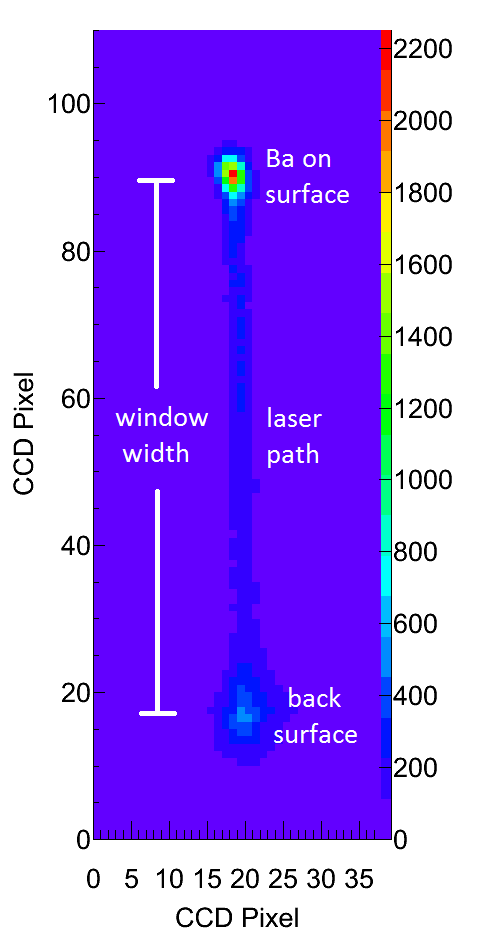
\includegraphics[width=.4\textwidth]{figures/raw_14-atom_labels_from_paper_1f.png}
                \caption{Example image of focused laser spot on sapphire window surface,and its path through the window.  \emph{\color{red}will replace w/ one w/o Ba}}
\label{fig:imageexamp}
\end{figure}

An example image of the focused 570~nm dye laser passing through a c-plane sapphire window of thickness 0.5~mm, using the 620-nm band-pass filter on the fluorescence, is shown in Fig. \ref{fig:imageexamp}.  With 4$\times$ magnification, each pixel is 5~$\mu$m$\times$5~$\mu$m.  The laser's path through the window is faintly visible by the tail of the broad Cr\textsuperscript{3+} fluorescence in the 620-nm band-pass.  The laser is focused at the top surface of the window, which faces the ion beam.  The surface background is seen on both surfaces.  The observed size of the laser spot, with a 1/e$^{2}$ radius of about 12~$\mu$m, is larger than the 2.06~$\mu$m $\times$ 2.66~$\mu$m 1/e$^{2}$ laser spot size.  Aberrations and vibrations in the collection optics could contribute to this inability to reach the diffraction limit in imaging.

%\begin{wrapfigure}{r}{0.5\textwidth}
  %\begin{center}
   % 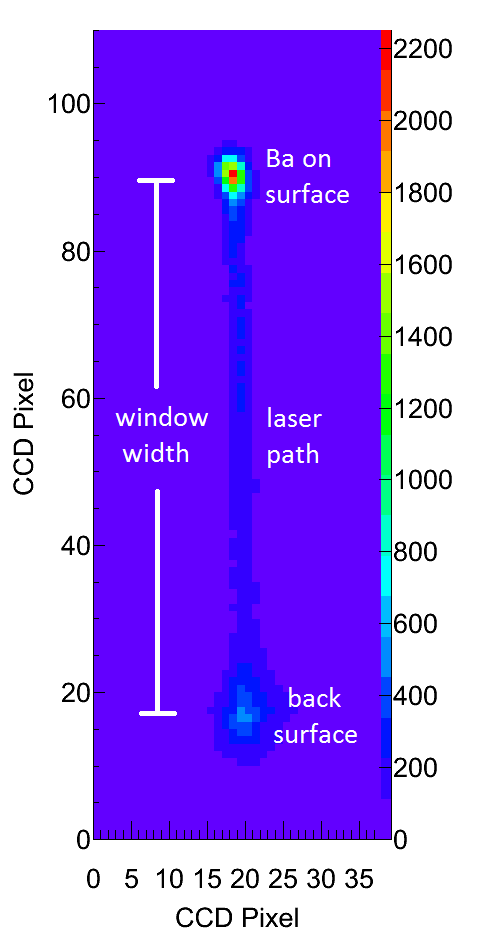
\includegraphics[width=0.35\textwidth]{figures/raw_14-atom_labels_from_paper_1f.png}
  %\end{center}
  %\caption{}
  %\label{fig:imageexamp}
%\end{wrapfigure}

\section{Vibrations and Effective Laser Region}

\begin{figure} %[H]
        \centering
                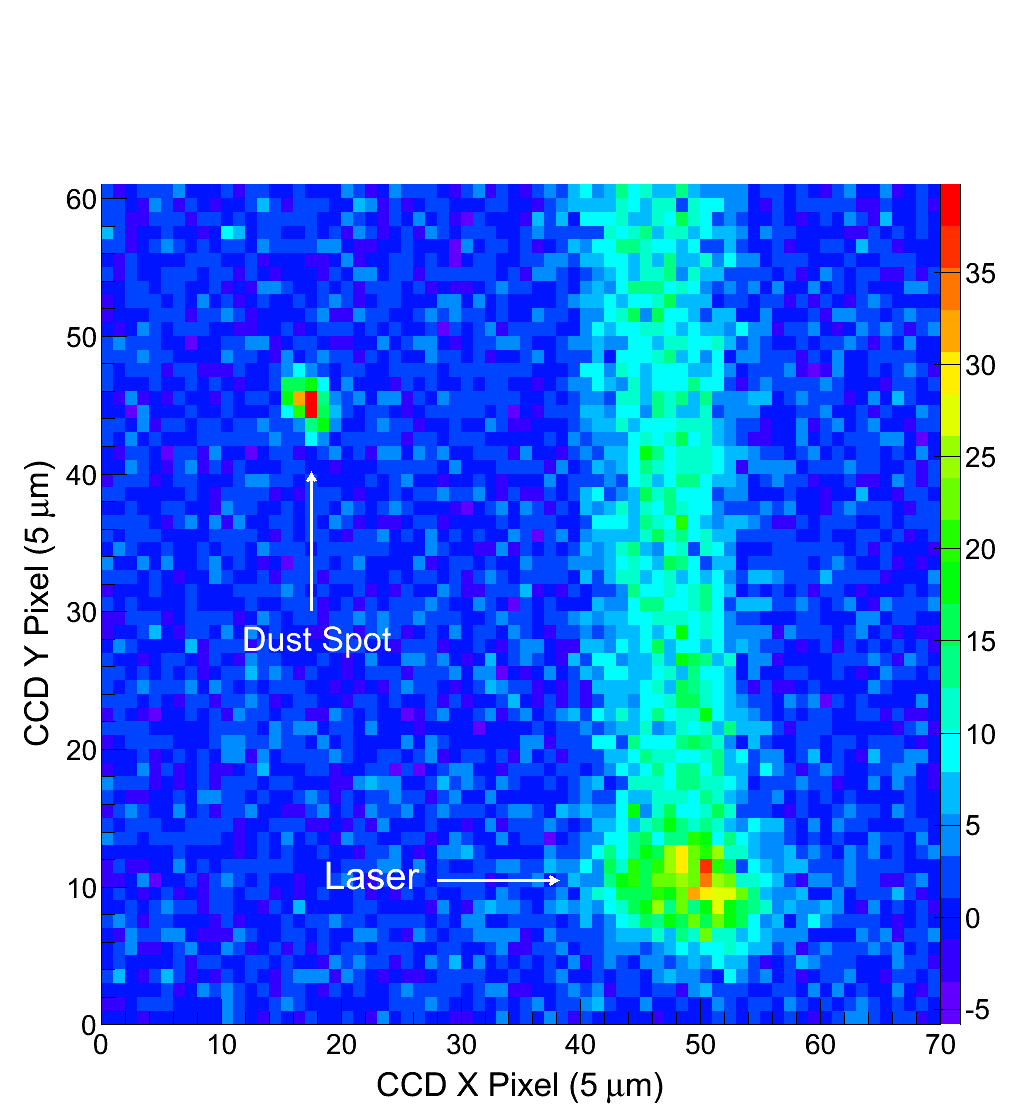
\includegraphics[width=.6\textwidth]{figures/image_dustspot.png}
                \caption{Example image of dust spot and laser during observation of cryostat vibrations.}
\label{fig:dustspot}
\end{figure}

Relative vibrations between the laser and sapphire window will affect the number of Ba atoms exposed, increasing the effective laser spot size.  This was studied by observing the position of a ``dust spot" (a highly scattering feature on the sapphire window) relative to the position of the laser in an image on time scales down to 50~ms.  An example of an image from this experiment is shown in Fig. \ref{fig:dustspot}.  The 570-nm dye laser was somewhat de-focused, and the dust spot was illuminated by a de-focused 657~nm diode laser. For each frame, 2D Gaussian functions were fit to locate the center of the laser spot and the dust spot in order to measure their relative position.  The fit for the laser spot was restricted in y so that it was not affected by the bulk sapphire fluorescence path.  The distances in x and y between the dust spot and laser are plotted for each 50-ms snapshot in Fig. \ref{fig:cryovibe2D}(a).  The distribution shows a correlation between x and y.  To calculate an effective laser spot size due to this vibration, each difference (x,y) between laser and dust spot was used as the center of a 2D Gaussian, each with w$_{x} = 2.06~\mu$m and w$_{y} = 2.66~\mu$m to represent the laser spot.  Such Gaussian functions were summed to all points to produce a distribution of summed laser exposure, shown in Fig. \ref{fig:cryovibe2D}{\color{red}(b)}.  The total area enclosed by a 1/e contour then represents the effective area.  Since x and y movement are correlated, and since the movement is sinusoidal, the effective area is only about 2$\times$ the real laser spot size, and the effective laser region is 17.8~$\mu$m$^{2}$.

%The difference between dust spot and laser positions is plotted in {\color{red}Fig. [fig vibe vs. time with sine fit]} for both x and y.  Each exposure in this plot is 50~ms, though readout time and camera shutter compensation time result in x~s between frames.  The best fit of a sine function results in a vibration frequency of x~Hz.  This is consistent with the audible frequency of the cryostat He pump.
%...could do this for rotated

\begin{figure} %[H]
        \centering
                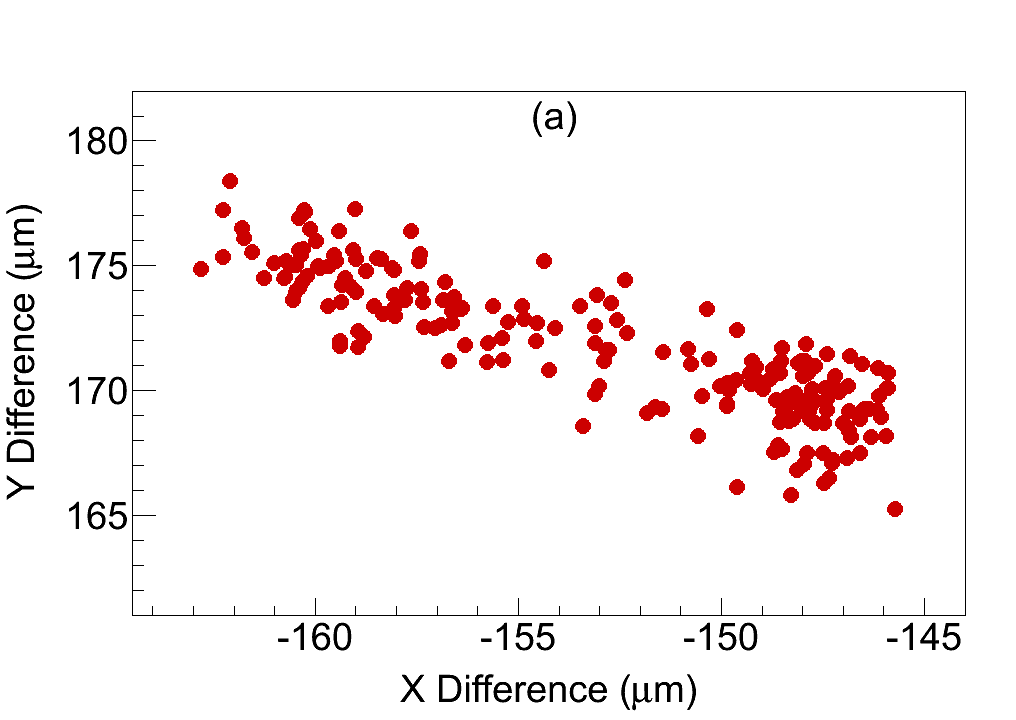
\includegraphics[width=.5\textwidth]{figures/cryovibes_a.png}
                ~
                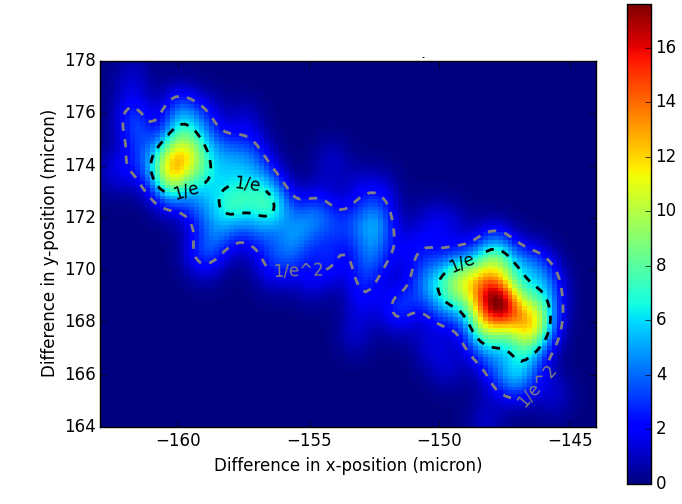
\includegraphics[width=.5\textwidth]{figures/cryovibes_b_chris_run10_15_diff_func_wcontour.png}
                \caption{Cryostat vibration measurements based on relative position of dust spot vs. laser on sapphire window in 50-ms snapshots (a), with 2D Gaussians overlain on each point to represent total laser exposure vs. position (b). \emph{\color{red}will re-do (b) myself}}
\label{fig:cryovibe2D}
\end{figure}

The aforementioned is the most concerning vibration to understand.  Vibration of the laser itself is included in that study.  Vibration of the collection optics will affect the imaging resolution, but not the number of atoms being observed.  These vibrations were minimized by stable mounts.

\section{Imaging 577- and 591-nm peaks}
\label{sec:imaging590and577}

\begin{figure} %[H]
        \centering
                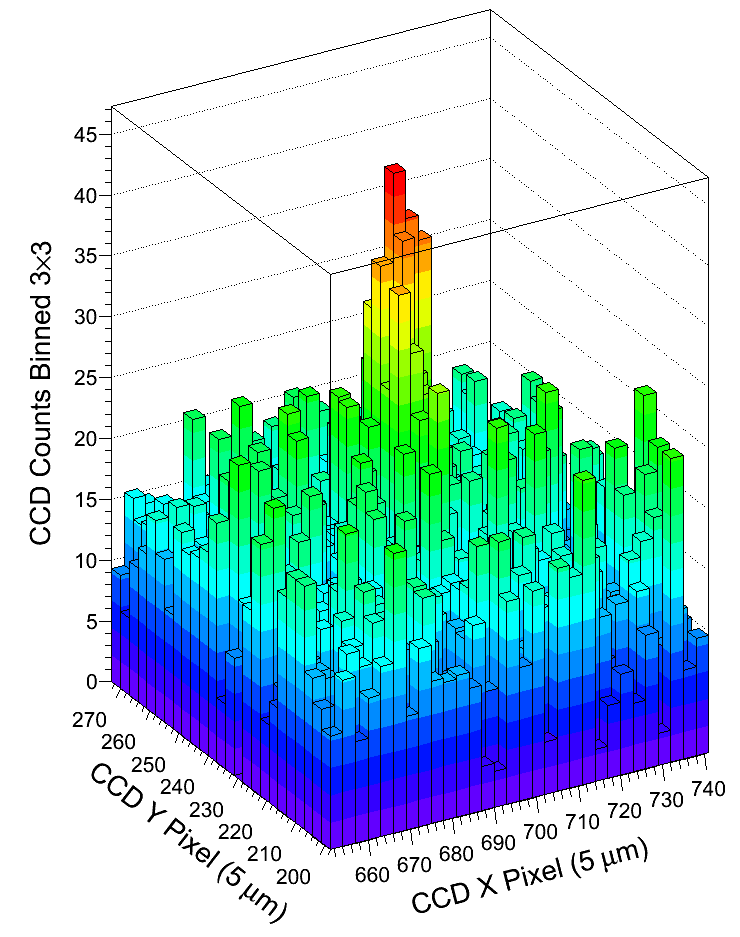
\includegraphics[width=.6\textwidth]{figures/image_1e4.png}
                \caption{Image of about $10^{4}$ total Ba atoms in SXe, with about $5 \times 10^{3}$ atoms exposed at a time.  100-s exposure with .02~$\mu$W of 566~nm excitation, deposited at 50~K and observed at 11~K.  $3 \times 3$ CCD pixel binning.}
\label{fig:image590s}
\end{figure}

First attempts at imaging small numbers of Ba atoms in a focused laser region were done with the 577- and 591-nm Ba fluorescence peaks together using a 586-nm band-pass filter, which passes 573 - 599~nm FWHM.  This filter has a 2" diameter, resulting in a factor of 4$\times$ more collection efficiency.  Bleaching data was used to optimize laser intensity and exposure time to achieve maximal signal in frame 1, and to avoid hole bleaching.  The fast bleaching of these peaks is the limiting factor on sensitivity.  An image of $\leq$ 10$^{4}$ atoms (10$^{4}$ Ba\textsuperscript{+} ions deposited into the effective laser region) is shown in Fig. \ref{fig:image590s}.  This is a 100-s exposure with 0.02~$\mu$W of 566-nm excitation.  At this low intensity, no bleaching was observed in the four frames observed (frame 1 is shown).  Since the effective laser region is approximately doubled by cryostat vibrations, the signal observed at a given moment in time is actually due to the real laser spot size in the scenario of little to no bleaching.  Thus it should be said that Fig. \ref{fig:image590s} is an image of $5 \times 10^{3}$ atoms on average, with $10^{4}$ total atoms exposed.  Groups of 9 ($3 \times 3$) CCD pixels are binned to produce the nice peak shown.  As discussed in \ref{sec:bleaching}, detection of very small numbers of atoms in these sites may require several infrared re-pump lasers.  As a result of low total exposure, neither the sapphire nor the surface backgrounds are present in these images, though a Xe-only image has been subtracted. 

\section{Imaging 619-nm peak}

\begin{figure} %[H]
        \centering
                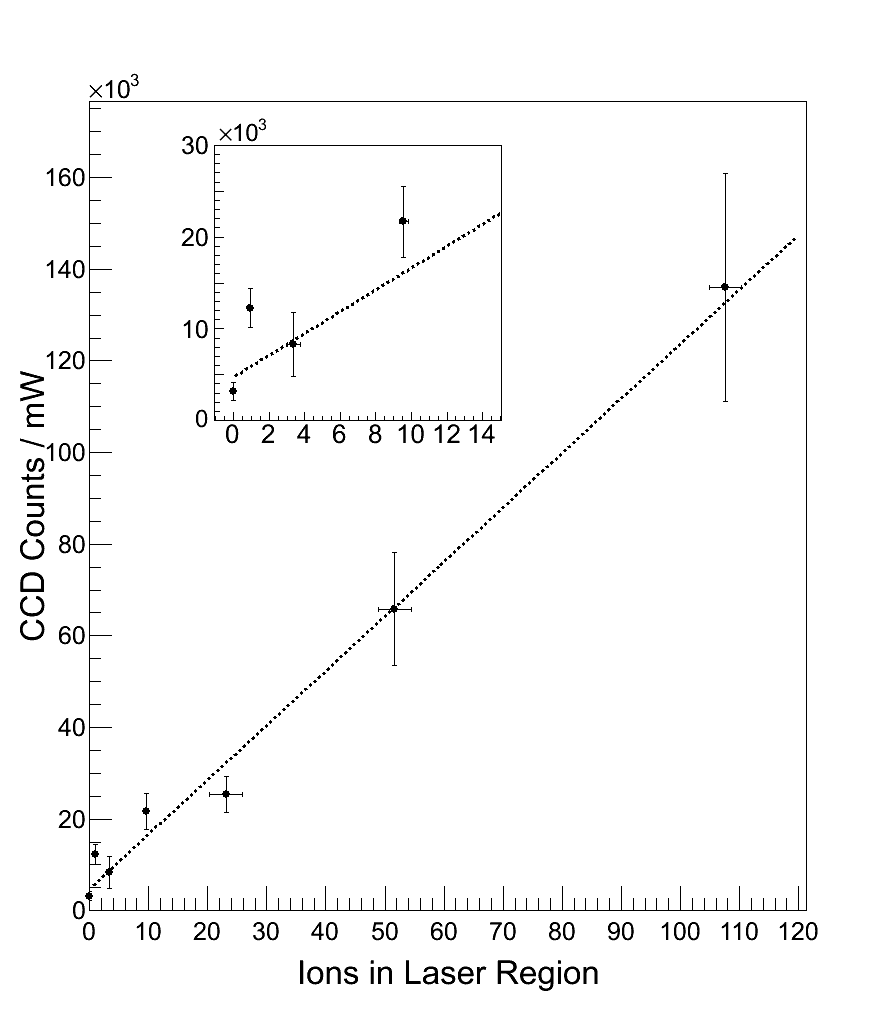
\includegraphics[width=.99\textwidth]{figures/fitgrouped_20150807_20150916_inset.png}
                \caption{619-nm signal vs. Ba\textsuperscript{+} deposited in effective excitation region of 17.8~$\mu$m using focused laser at 570~nm. \emph{\color{red}move y-ax title over, Remove x errors}}
\label{fig:lin}
\end{figure}

At low laser intensities, the 619-nm peak appears minor compared to the 577- and 591-nm peaks.  However, its much lower bleaching rate brings it to dominate over larger exposures, e.g. with the intensity of a focused laser at 0.01-0.1~mW over seconds or minutes.  Experiments imaging small numbers of Ba atoms in SXe in a focused laser region with the 619-nm peak were successful down to the single-atom level.

\begin{figure} %[H]
        \centering
                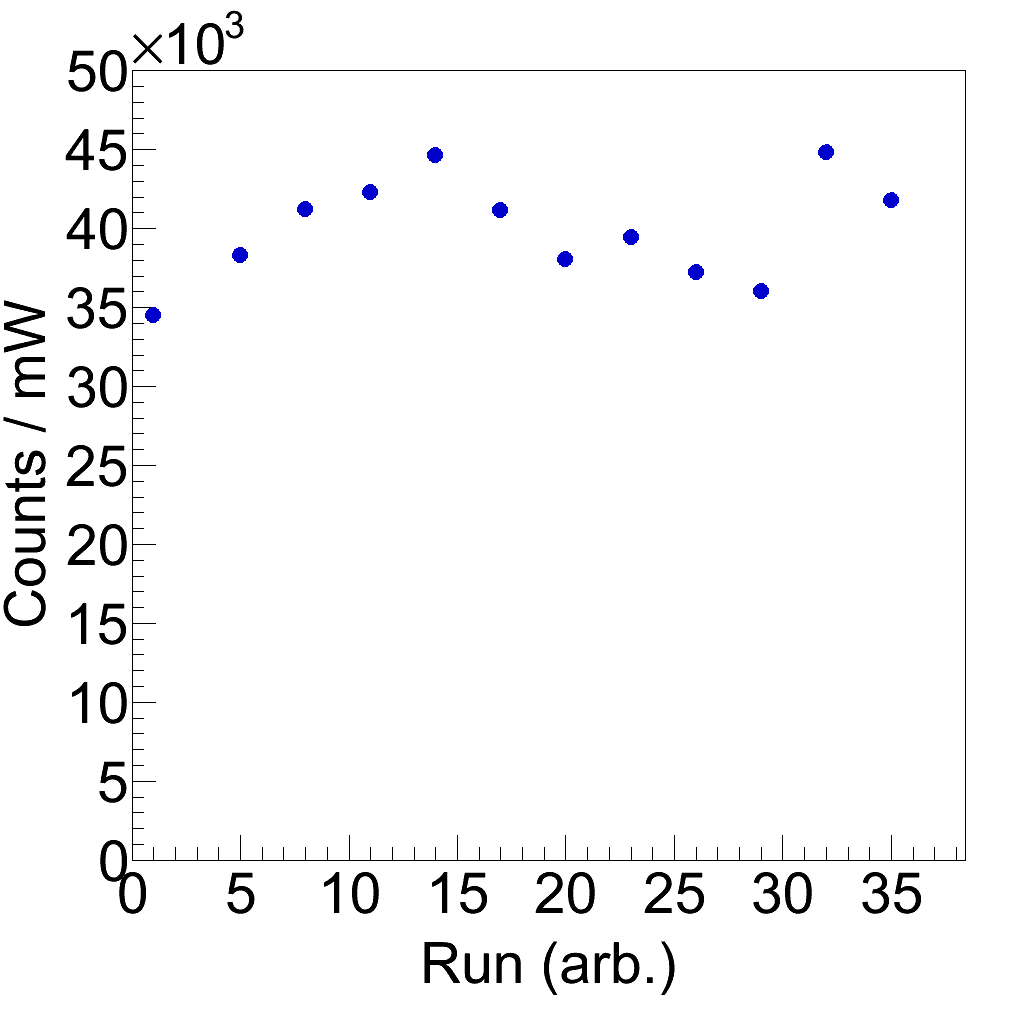
\includegraphics[width=.4\textwidth]{figures/xe_variation.png}
                \caption{Background counts in focused laser region over the course of an experiment.}
\label{fig:xevar}
\end{figure}

An imaging experiment consisted of many different pulsed Ba\textsuperscript{+} deposits, each of which was evaporated after observation.  This procedure is described in \ref{sec:deposition}-\ref{sec:collection}.  A linear relationship between observed signal and ions deposited must be observed and repeated.  Frequent Xe-only deposits ware made, typically every three runs, to establish the local background.  The image of each deposit was analyzed by summing the counts of a 3-pixel$\times$3-pixel (15$\mu$m$\times$15$\mu$m) region centered on the laser spot in the SXe layer where it excites Ba atoms, i.e. at the top of the laser path in Fig. \ref{fig:imageexamp}.  A partial-bin integrator was implemented such that the 3-pixel$\times$3-pixel region could be centered on the peak center of each run, which typically varied by about half a micron between runs.  Summed counts vs. Ba\textsuperscript{+} ions deposited into the laser region is shown in Fig. \ref{fig:lin} for a combination of data sets from two separate days \emph{\color{blue}maybe you want them separate (with each point having errors) by color to show agreement }  Each point has subtracted the averaged counts from the two surrounding Xe-only deposits.  Some variation in signal is observed, likely due to spatial drifting of the ion beam, as this variation was larger on days where larger beam drift was observed.  Nonetheless, a clear linearity in observed in signal vs. ions deposited, all the way down to single ions deposited.  Recall that the number of ions is an upper limit on the number of atoms in the 619-nm peak matrix site.  ``0-pulse" deposits are also made, wherein Faraday cup 3 is retracted for the 1-s period, but the ion beam remains deflected with no pulses.  This establishes the level of neutral Ba atoms making their way down the beam line from the source into the laser region.  Signal at the few-atom level is observed from these deposits.

%... and try combining those other days.  It will require scaling for intensity difference (spher. abb.) and time, and remember different I$\times$t might give different efficiency.

\begin{figure} %[H]
        \centering
                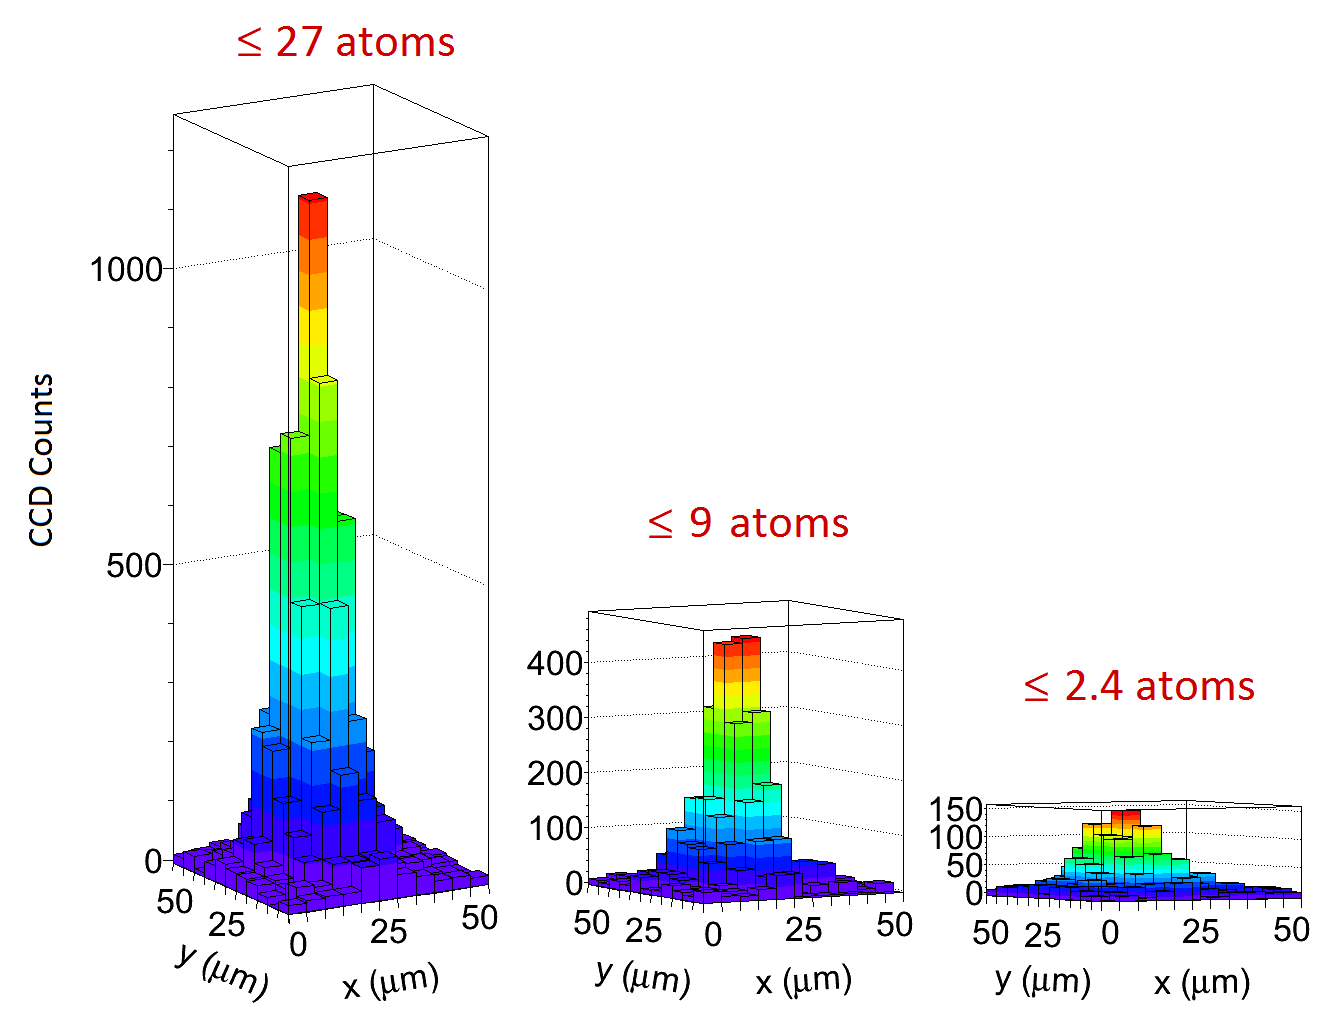
\includegraphics[width=.99\textwidth]{figures/train_20150807_v3_runs70_88_81_fromGiorgioFolder.png}
                \caption{\color{red}will change:  1) have more than this, 2) do pixel (5micron) on axis like others, 3) have same-looking phi angle on all}
\label{fig:train}
\end{figure}

\begin{figure} %[H]
        \centering
                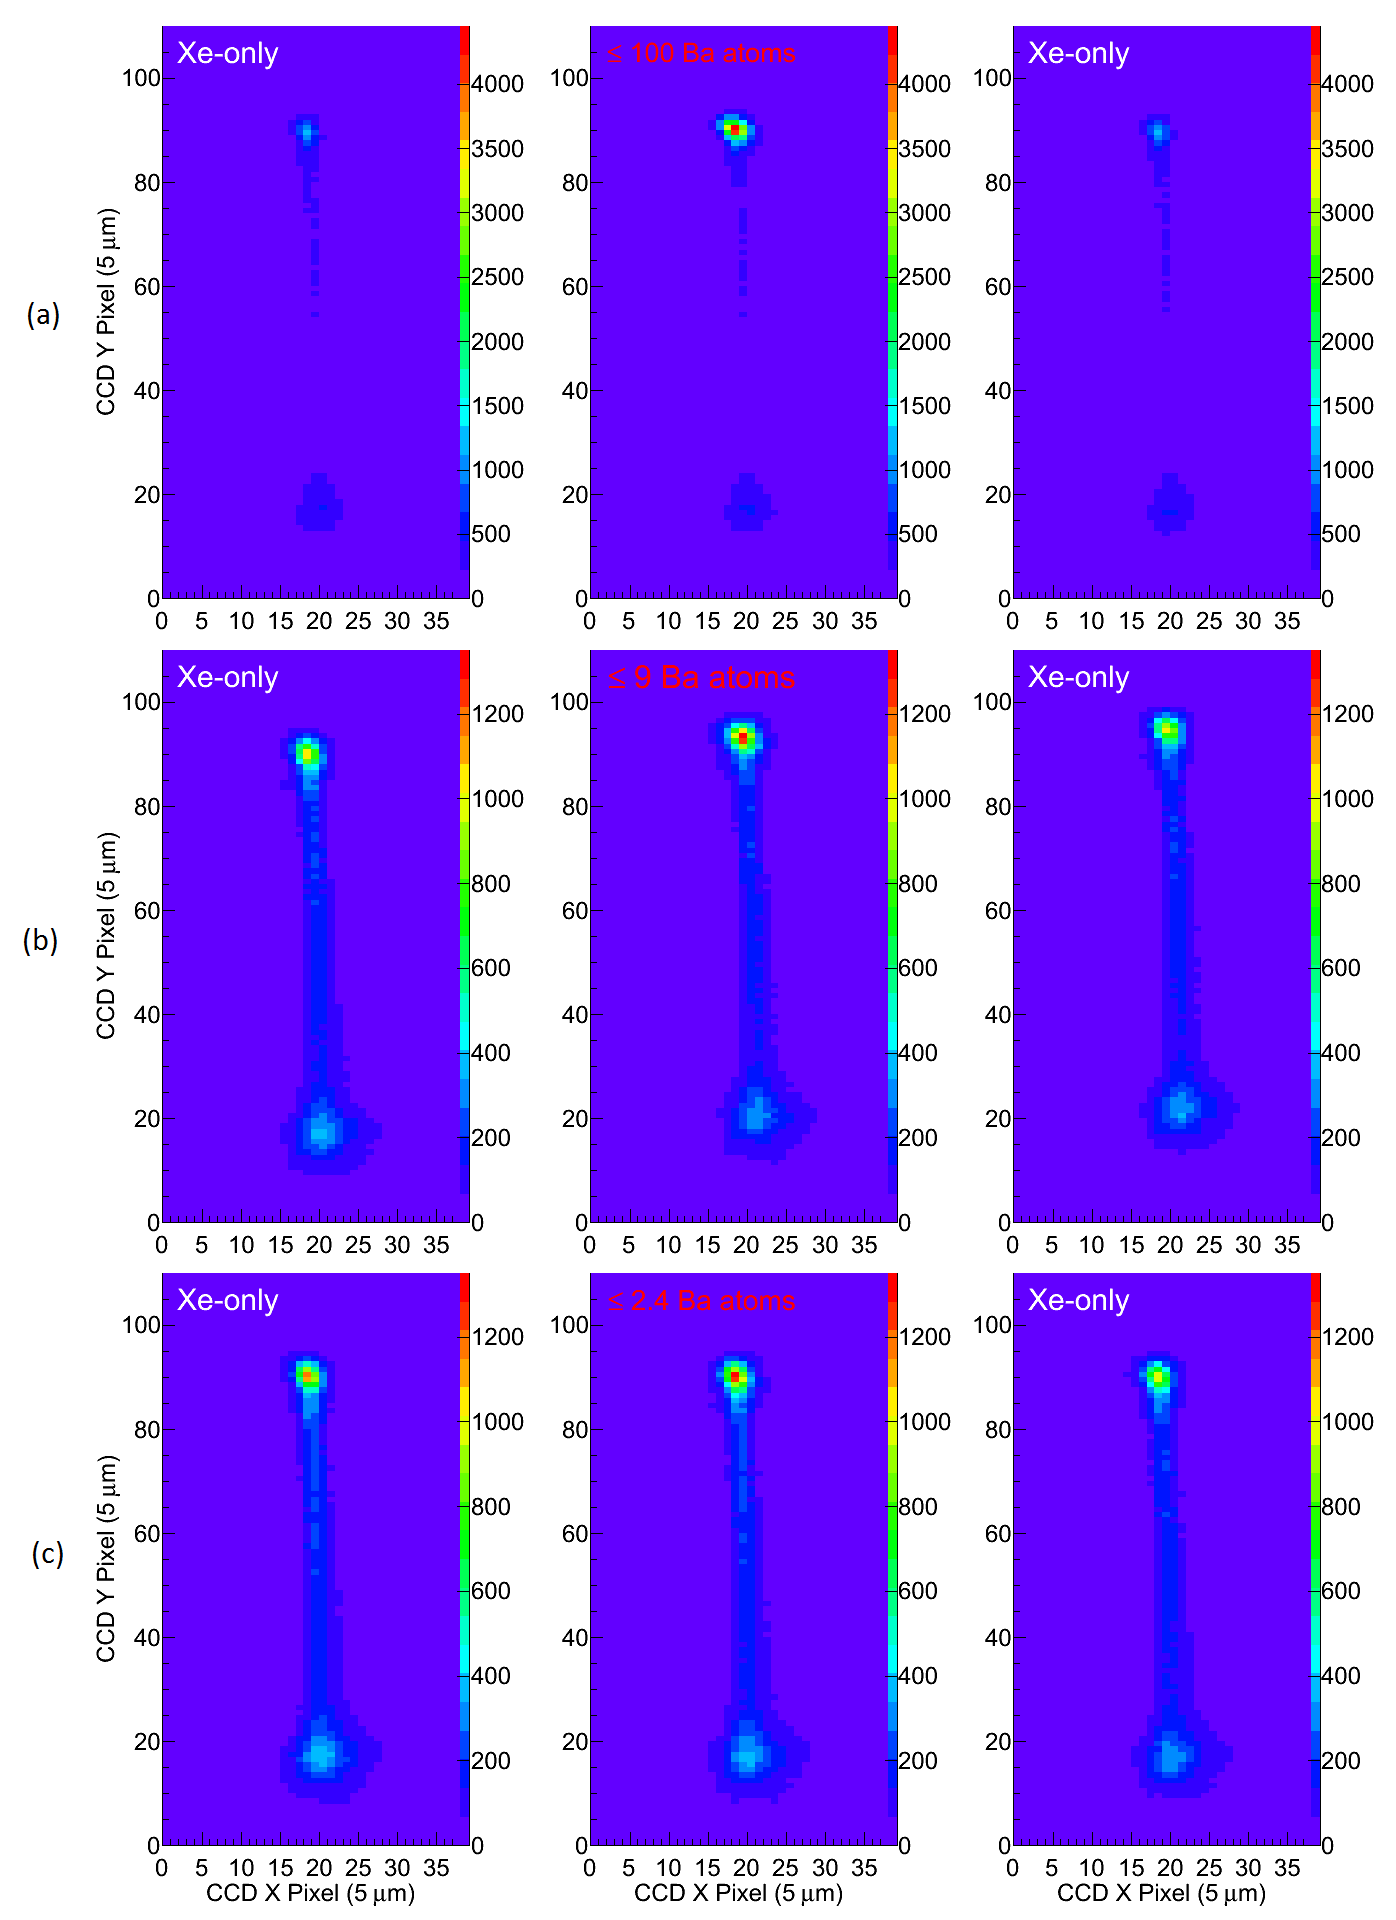
\includegraphics[width=.95\textwidth]{figures/xebaxe.png}
                \caption{Raw images of three Ba\textsuperscript{+} deposits yielding (a) $\leq 100$, (b) $\leq 9$, and (c) $\leq 2.4$ Ba atoms, with their preceding and succeeding Xe-only deposits.}
\label{fig:xebaxe}
\end{figure}

Variation in the background level, dominated by the surface background, is shown in Fig. \ref{fig:xevar}.  Variation was most likely caused by drift of the laser position on the window, to regions of different historical bleaching.  Local variations are at the single-atom signal level, however positive signal after subtraction, even at the single-atom level, demonstrates that this variation is sufficiently low.

Xe-only images were also directly subtracted to produce images of 619-nm Ba fluorescence.  In cases where the image has shifted slightly between runs, a binning redistribution was applied to do sub-pixel image shifting for better subtraction, though images which did not require this were preferred.  619-nm fluorescence images for several deposits of varying numbers of atoms are shown in Fig. \ref{fig:train}.  

It is important to note that no Ba signal is left behind after a sample is evaporated, even for large Ba\textsuperscript{+} deposits.  Raw images (pedestal-subtracted) of Ba\textsuperscript{+} deposits and their preceding and succeeding Xe-only deposits are shown in Fig. \ref{fig:xebaxe} for several runs.  The lack of historical buildup of Ba is important for the implementation of this method of Ba tagging on a probe in nEXO.

\section{Scanned Images}
\label{sec:scanning}

The ultimate demonstration of single-atom imaging would be to scan the focused laser over a sample of separated Ba atoms, observing a peak when the laser moves over each atom.  Preliminary scans were performed by scanning the focusing lens in a grid patter, using the setup described in \ref{sec:laserscanning}.   \emph{\color{gray}choose what to show and what to say about it -- there are some decent things to show really}  [issues are BG, reproduceability, vibrations]
